\section{Auswertung}

Zunächst werden die Kennlinien bei verschiedenen Heizleistungen bestimmt. Da
die Temperatur nicht gemessen werden kann wird die Stromstärke und Spannung notiert. Die
Messwerte der einzelnen Messungen sind in Tabelle \ref{tab:1} dargestellt.

\begin{table}[H]
  \centering
  \caption{Messwerte der Messungen für die Kennlinien.}
  \label{tab:1}
  \begin{tabular}{c c c c c c c c c c}
\toprule
\multicolumn{2}{c}{$I=\SI{1.8}{\ampere}$} & \multicolumn{2}{c}{$I=\SI{1.9}{\ampere}$} & \multicolumn{2}{c}{$I=\SI{2.0}{\ampere}$} & \multicolumn{2}{c}{$I=\SI{2.2}{\ampere}$} & \multicolumn{2}{c}{$I=\SI{2.4}{\ampere}$}\\
\cmidrule(lr){1-2}\cmidrule(lr){3-4}\cmidrule(lr){5-6}\cmidrule(lr){7-8}\cmidrule(lr){9-10}
$U \, / \, \si{\volt}$ & $I \, / \, \si{\milli\ampere}$ & $U \, / \, \si{\volt}$ & $I \, / \, \si{\milli\ampere}$ &$U \, / \, \si{\volt}$ & $I \, / \, \si{\milli\ampere}$ & $U \, / \, \si{\volt}$ & $I \, / \, \si{\milli\ampere}$ & $U \, / \, \si{\volt}$ & $I \, / \, \si{\milli\ampere}$ \\
\midrule
0   & 0,000 & 0   & 0,000 & 0   & 0,000 & 0   & 0,000 & 0   & 0,000 \\
5   & 0,001 & 5   & 0,000 & 5   & 0,000 & 5   & 0,013 & 2   & 0,004 \\
10  & 0,008 & 10  & 0,000 & 10  & 0,004 & 10  & 0,053 & 4   & 0,016 \\
15  & 0,013 & 15  & 0,003 & 15  & 0,023 & 15  & 0,108 & 6   & 0,033 \\
20  & 0,014 & 20  & 0,011 & 20  & 0,044 & 20  & 0,166 & 8   & 0,067 \\
25  & 0,015 & 25  & 0,023 & 25  & 0,066 & 25  & 0,236 & 10  & 0,088 \\
30  & 0,016 & 30  & 0,031 & 30  & 0,080 & 30  & 0,285 & 12  & 0,122 \\
35  & 0,016 & 35  & 0,035 & 35  & 0,086 & 35  & 0,331 & 14  & 0,150 \\
40  & 0,016 & 40  & 0,037 & 40  & 0,089 & 40  & 0,358 & 16  & 0,180 \\
45  & 0,017 & 45  & 0,038 & 45  & 0,091 & 45  & 0,376 & 18  & 0,217 \\
50  & 0,017 & 50  & 0,039 & 50  & 0,092 & 50  & 0,387 & 20  & 0,250 \\
55  & 0,017 & 55  & 0,039 & 55  & 0,093 & 55  & 0,394 & 22  & 0,290 \\
60  & 0,017 & 60  & 0,040 & 60  & 0,095 & 60  & 0,400 & 24  & 0,332 \\
70  & 0,017 & 70  & 0,040 & 70  & 0,095 & 70  & 0,407 & 26  & 0,366 \\
80  & 0,017 & 80  & 0,041 & 80  & 0,096 & 80  & 0,411 & 28  & 0,407 \\
90  & 0,017 & 90  & 0,041 & 90  & 0,096 & 90  & 0,414 & 30  & 0,453 \\
100 & 0,017 & 100 & 0,041 & 100 & 0,097 & 100 & 0,417 & 32  & 0,499 \\
110 & 0,018 & 110 & 0,041 & 110 & 0,097 & 110 & 0,419 & 34  & 0,545 \\
120 & 0,018 & 120 & 0,042 & 120 & 0,098 & 120 & 0,422 & 36  & 0,585 \\
130 & 0,018 & 130 & 0,042 & 130 & 0,098 & 130 & 0,423 & 38  & 0,625 \\
140 & 0,018 & 140 & 0,042 & 140 & 0,099 & 140 & 0,425 & 40  & 0,660 \\
150 & 0,018 & 150 & 0,042 & 150 & 0,099 & 150 & 0,427 & 42  & 0,699 \\
160 & 0,018 & 160 & 0,043 & 160 & 0,099 & 160 & 0,428 & 44  & 0,735 \\
170 & 0,018 & 170 & 0,043 & 170 & 0,100 & 170 & 0,430 & 46  & 0,768 \\
180 & 0,018 & 180 & 0,043 & 180 & 0,100 & 180 & 0,431 & 48  & 0,808 \\
190 & 0,018 & 190 & 0,043 & 190 & 0,100 & 190 & 0,432 & 50  & 0,852 \\
200 & 0,018 & 200 & 0,043 & 200 & 0,100 & 200 & 0,433 & 52  & 0,891 \\
210 & 0,018 & 210 & 0,043 & 210 & 0,101 & 210 & 0,434 & 54  & 0,921 \\
220 & 0,018 & 220 & 0,043 & 220 & 0,101 & 220 & 0,435 & 56  & 0,959 \\
230 & 0,018 & 230 & 0,043 & 230 & 0,101 & 230 & 0,436 & 58  & 0,983 \\
240 & 0,018 & 240 & 0,044 & 240 & 0,101 & 240 & 0,437 & 60  & 1,013 \\
250 & 0,018 & 250 & 0,044 & 250 & 0,102 & 250 & 0,438 & 70  & 1,165 \\
 -  &   -   &  -  &   -   &  -  &   -   &  -  &   -   & 80  & 1,274 \\
 -  &   -   &  -  &   -   &  -  &   -   &  -  &   -   & 90  & 1,341 \\
 -  &   -   &  -  &   -   &  -  &   -   &  -  &   -   & 100 & 1,406 \\
 -  &   -   &  -  &   -   &  -  &   -   &  -  &   -   & 110 & 1,438 \\
 -  &   -   &  -  &   -   &  -  &   -   &  -  &   -   & 120 & 1,463 \\
 -  &   -   &  -  &   -   &  -  &   -   &  -  &   -   & 130 & 1,481 \\
 -  &   -   &  -  &   -   &  -  &   -   &  -  &   -   & 140 & 1,491 \\
 -  &   -   &  -  &   -   &  -  &   -   &  -  &   -   & 150 & 1,501 \\
 -  &   -   &  -  &   -   &  -  &   -   &  -  &   -   & 160 & 1,507 \\
 -  &   -   &  -  &   -   &  -  &   -   &  -  &   -   & 170 & 1,514 \\
 -  &   -   &  -  &   -   &  -  &   -   &  -  &   -   & 180 & 1,520 \\
 -  &   -   &  -  &   -   &  -  &   -   &  -  &   -   & 190 & 1,524 \\
 -  &   -   &  -  &   -   &  -  &   -   &  -  &   -   & 200 & 1,530 \\
 -  &   -   &  -  &   -   &  -  &   -   &  -  &   -   & 210 & 1,534 \\
 -  &   -   &  -  &   -   &  -  &   -   &  -  &   -   & 220 & 1,538 \\
 -  &   -   &  -  &   -   &  -  &   -   &  -  &   -   & 230 & 1,542 \\
 -  &   -   &  -  &   -   &  -  &   -   &  -  &   -   & 240 & 1,545 \\
 -  &   -   &  -  &   -   &  -  &   -   &  -  &   -   & 250 & 1,550 \\
\bottomrule
  \end{tabular}
\end{table}

Die Messwerte sind in Abbildung \ref{abb:6} Graphisch dargestellt.

\begin{figure}[H]
  \centering
  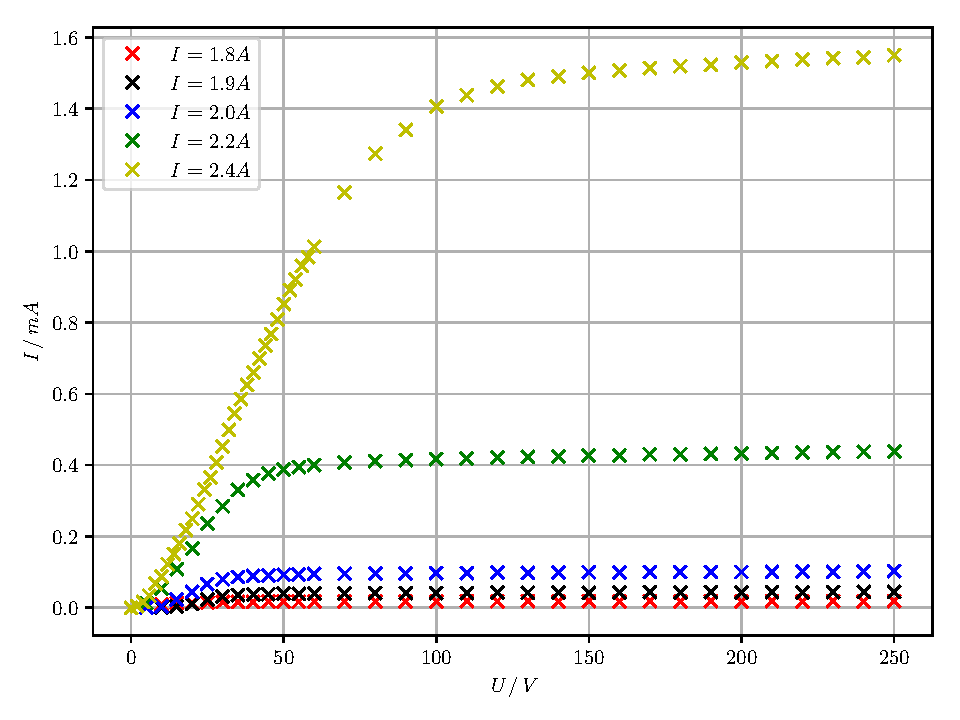
\includegraphics{plot1.pdf}
  \caption{Graphische Darstellung der Kennlinien.}
  \label{abb:6}
\end{figure}

Aus der graphischen Darstellung der Messwerte lässt sich nun der Sättigungsstrom
$I_s$ ablesen. Der Sättigungsstrom für die einzelnen Stromstärken sind in Tabelle
\ref{tab:2} dargestellt.

\begin{table}[H]
  \centering
  \caption{Sättigungsstrom für die einzelnen Stromstärken.}
  \label{tab:2}
  \begin{tabular}{c c}
    \toprule
    $I \, / \, \si{\ampere}$ & $I_s \, / \, \si{\milli\ampere}$ \\
    \midrule
    1,8 & 0,018  \\
    1,9 & 0,044  \\
    2,0 & 0,102  \\
    2,2 & 0,438  \\
    2,4 & 1,550  \\
    \bottomrule
  \end{tabular}
\end{table}

Als nächstes wird das Raumladungsgebiet für die maximale Heizleistung, bei $\SI{2.4}{\ampere}$,
untersucht. Dazu werden die Messwerte aus Tabelle \ref{tab:1} aus dem Raumladungsgebiet, in der Abbildung \ref{abb:7},
Graphisch dargestellt. Das Raumladungsgebiet geht bis $\SI{60}{\volt}$.
Mit diesen Messwerten wird nun eine Ausgleichsrechnung durchgeführt mit Python 3.6.
Die verwendete Gleichung dabei lautet

\begin{equation*}
  I(U) = a \cdot U^b.
\end{equation*}

Es wird der Exponent der Strom-Spannung Beziehung bestimmt.

\begin{figure}[H]
  \centering
  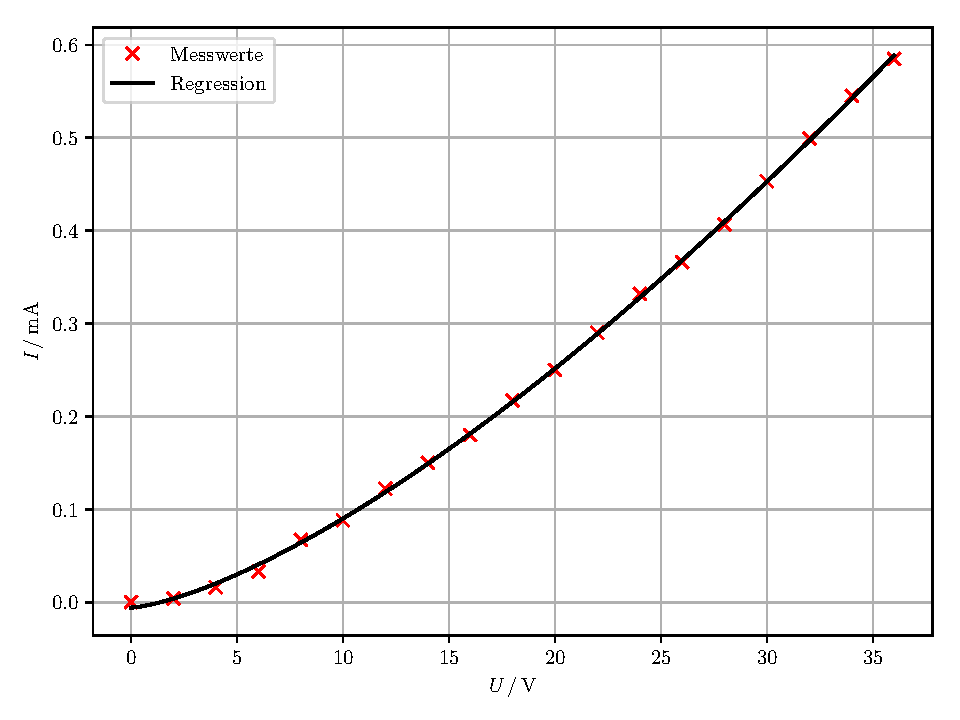
\includegraphics{plot2.pdf}
  \caption{Darstellung des Raumladungsgebiets und der Ausgleichsrechnung.}
  \label{abb:7}
\end{figure}

Damit ergeben sich die Parameter zu:

\begin{equation*}
  b = \num{1.425(16)}
\end{equation*}
\begin{equation*}
  a = \num{3.61(21)e-3}
\end{equation*}


Daraufhin wird das Anlaufstromgebiet untersucht, welches von der Gleichung \ref{eq:1} beschrieben wird.
Die Messwerte dieser Messung sind
in der Tabelle \ref{tab:3} dargestellt. Da es einen Spannungsabfall am Innenwiderstand des
Nanoamperemeter, der $\SI{1}{\mega\ohm}$ beträgt, gibt müssen die gemessenen Spannungswerte
korrigiert werden mit der folgenden Gleichung

\begin{equation*}
  U_\text{korr} = U - R_\text{innen} I.
\end{equation*}

\begin{table}[H]
  \centering
  \caption{Messwerte für das Anlaufstromgebiet.}
  \label{tab:3}
  \begin{tabular}{c c c}
    \toprule
    $ U \, / \, \si{\volt}$ & $U_\text{korr} \, / \, \si{\volt}$ & $ I \, / \, \si{\nano\ampere}$ \\
    \midrule
    0,0 & -0,135 & 135,0 \\
    0,1 & -0,005 & 105,0 \\
    0,2 &  0,121 &  79,0 \\
    0,3 &  0,244 &  56,0 \\
    0,4 &  0,360 &  40,0 \\
    0,5 &  0,480 &  20,0 \\
    0,6 &  0,582 &  18,5 \\
    0,7 &  0,689 &  11,5 \\
    0,8 &  0,793 &   7,0 \\
    0,9 &  0,896 &   4,4 \\
    1,0 &  0,997 &   2,6 \\
    \bottomrule
  \end{tabular}
\end{table}

Die ersten beiden Werte durch die Korrektur negativ werden, werden diese bei der
Ausgleichsrechnung nicht betrachtet. Diese Werte liegen nicht mehr im Anlaufstromgebiet.
Mit Hilfe dieser Messwerte wird nun die Temperatur $T$ der Kathode bestimmt.
Dazu wird die folgende Gleichung verwendet um eine Ausgleichsrechnung durchzuführen:

\begin{equation*}
  I(U) = a \cdot \exp(-b U)
\end{equation*}

Diese Ausgleichsrechnung wird wieder mit Python 3.6 durchgeführt. Die Ergebnisse sind
in Abbildung \ref{abb:8} dargestellt.

\begin{figure}[H]
  \centering
  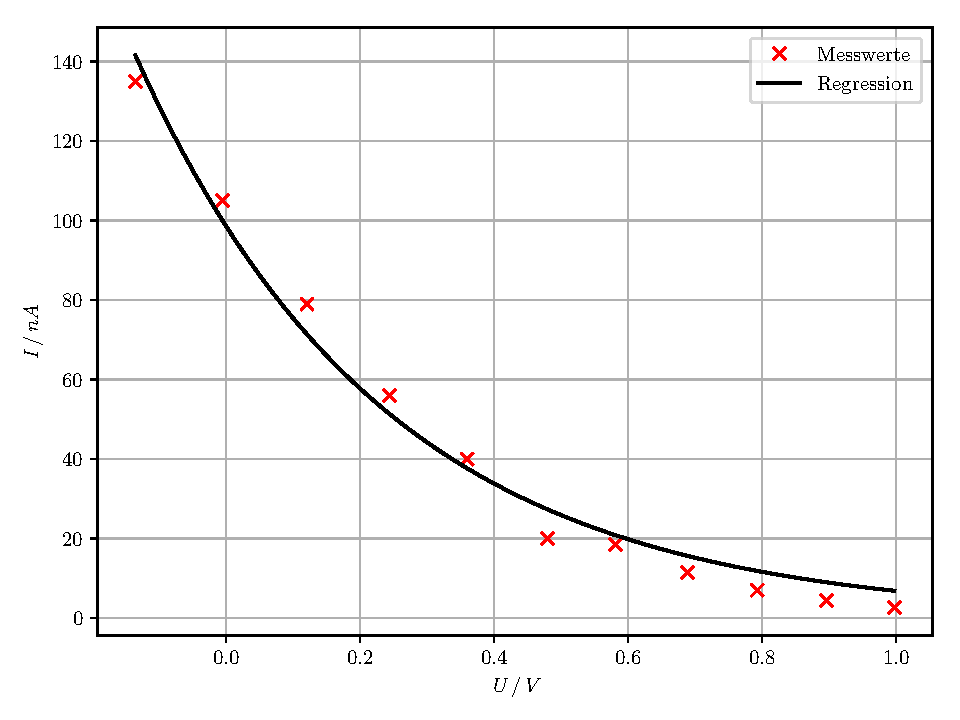
\includegraphics{plot3.pdf}
  \caption{Darstellung der Messwerte des Anlaufstromgebiet und der Ausgleichsrechnung.}
  \label{abb:8}
\end{figure}

Die Parameter ergeben sich somit zu:

\begin{equation*}
  a = \SI{121.79(548)}{\nano\ampere}
\end{equation*}
\begin{equation*}
  b = \SI{3.37(17)}{\per\volt}
\end{equation*}

Aus $b$ lässt sich nun die Temperatur bestimmen mithilfe der Gleichung \ref{eq:1}.

\begin{equation*}
  T = \frac{e_0}{k_b b}
\end{equation*}

Der Fehler wird mit der Gauß´schen Fehlerfortpflanzung bestimmt:

\begin{equation*}
  \Delta T = \sqrt{\left(-\frac{e_0}{k_b b^2}\right)^2 \cdot (\Delta b)^2}
\end{equation*}

Die Temperatur ergibt sich somit zu

\begin{equation*}
  T = \SI{3440(170)}{\kelvin}.
\end{equation*}

Nun wird die Temperatur bei denen die einzelnen Kennlinien bestimmt wurden mittels
einer Leistungsbilanz bestimmt. Die aus dem Energiesatz hergeleitete Gleichung lautet

\begin{equation*}
  I_f U_f = f \eta \sigma T^4 + N_{WL}.
\end{equation*}

Dabei ist $f$ die emittierende Kathodenoberfläche $f = \SI{0.35}{\centi\meter\squared}$,
$\eta$ der Emissionsgrad $\eta = 0,28$, $\sigma$ ist die Strahlungskonstante $\sigma = \SI{5.7e-12}{\watt\per\centi\meter\kelvin\tothe{4}}$
und $N_{WL}$ ist die Wärmeleitung, die hier zu $N_{WL} = \SI{1}{\watt}$ abgeschätzt wird.

Die Messwerte von Strom und Spannung bei den einzelnen Kennlinien, sowie die
bestimmte Temperatur sind in Tabelle \ref{tab:4} gezeigt.

\begin{table}[H]
  \centering
  \caption{Darstellung der Messwerte von Strom und Spannung, sowie der Temperatur bei den einzelnen Kennlinien.}
  \label{tab:4}
  \begin{tabular}{c c c}
    \toprule
    $U \, / \, \si{\volt}$ & $I \, / \, \si{\ampere}$ & $T \, / \, \si{\kelvin}$ \\
    \midrule
    1,8 & 3,9 & 1852,91 \\
    1,9 & 4,0 & 1896,01 \\
    2,0 & 4,4 & 1976,87 \\
    2,2 & 5,0 & 2103,56 \\
    2,4 & 5,9 & 2253,04 \\
    \bottomrule
  \end{tabular}
\end{table}


Als letzte wird noch die Austrittsarbeit des Kathodenmaterials bestimmt. Dafür wird
die Gleichung \ref{eq:3} nach der Austrittsarbeit $e_0 \Phi$ umgeformt

\begin{equation*}
  e_0 \Phi = - k_b T \cdot \ln \left(\frac{I_s h^3}{4 \pi f e_0 m_0 k_b^2 T^2}\right).
\end{equation*}

Die Ergebnisse für die einzelnen Kennlinien sind in Tabelle \ref{tab:5} dargestellt.

\begin{table}[H]
  \centering
  \caption{Darstellung des Sättigungsströme, der Temperaturen und die Austrittsarbeiten.}
  \label{tab:5}
  \begin{tabular}{c c c}
    \toprule
    $I_s \, / \, \si{\milli\ampere}$ & $T \, / \, \si{\kelvin}$ & $e_0 \Phi \, / \, \si{\eV}$ \\
    \midrule
    0,018 & 1892,91 & 4,994 \\
    0,044 & 1896,01 & 4,974 \\
    0,102 & 1976,87 & 5,060 \\
    0,438 & 2103,56 & 5,148 \\
    1,550 & 2253,04 & 5,300 \\
    \bottomrule
  \end{tabular}
\end{table}

Aus den bestimmten Austrittsarbeiten wird nun der Mittelwert und die Standartabweichung
des Mittelwerts mit den folgenden Gleichungen bestimmt:

\begin{equation*}
    \overline{(e_0\Phi)} = \frac{1}{5} \sum_{i=1}^{5} (e_0\Phi)_i
\end{equation*}
\begin{equation*}
  \Delta \overline{(e_0\Phi)} = \frac{1}{\sqrt{5}\sqrt{4}} \sqrt{\sum_{i=1}^{4}\left((e_0\Phi)_i-\overline{(e_0\Phi)}\right)^2}
\end{equation*}


Damit ergibt sich die gemittelte Austrittsarbeit zu

\begin{equation*}
  \overline{(e_0\Phi)} = \SI{5.095(60)}{\eV}.
\end{equation*}
